\section{Lightweight Methods for Imbalanced Learning} \label{sec:methodology}

The proposed pipeline presents a novel approach to address class imbalance in machine learning. The process begins with the input of raw training data, which undergoes augmentation through a series of lightweight transformation techniques. 
%These techniques, including AutoRand, RandAug, Cutout, Mixup, and Sampling, generate diverse and representative training samples, ensuring that underrepresented classes receive adequate exposure during training. This enhancement step is crucial for reducing the bias inherent in unbalanced datasets, where certain classes have far more data than others.
% \ha{\textcolor{blue}{(RESOLVED) I temporarily leave the draft idea of our imbalanced learning method here. PLEASE HELP TO POLISH AND IMPROVE THE APPEARANCE OF IT !!!!}}
%Data augmentation leads to a more useful enriched training dataset, which serves as input for the imbalance learning phase.
In the learning stage, various strategies, such as reweighting, resampling, or class-balanced loss functions, can be applied to further enhance the performance of the model in minority classes. This step is critical in ensuring that the model does not simply memorize the majority class patterns but learns to generalize effectively across all categories. Finally, the trained model proceeds to the prediction phase, where it makes informed decisions based on the improved training distribution. The proposed ILWH combines Mixup-based sample interpolation with deferred re-weighting in a unified and lightweight manner. 
Since Mixup operates as a simple linear combination of input pairs within each mini-batch, it requires no auxiliary networks or additional forward--backward passes. 
Consequently, ILWH introduces less than $3\%$ runtime overhead compared to the ERM baseline, consistent with previous findings that Mixup-style methods are computationally efficient \cite{zhang2017Mixup}. 
Moreover, ILWH maintains the same number of trainable parameters as the backbone classifier, confirming that the method is structurally lightweight.

%This approach is motivated by the limitations of traditional imbalance-handling techniques, such as oversampling and cost-sensitive learning, which often introduce computational overhead or lead to overfitting. Unlike these conventional methods, lightweight data augmentation techniques offer an adaptive and computationally efficient solution to class imbalance. By introducing synthetic diversity, augmentations such as Mixup and RandAug prevent models from overfitting to specific class distributions and help smooth decision boundaries, thereby improving generalization.
\begin{figure}[htbp]
    \centering
    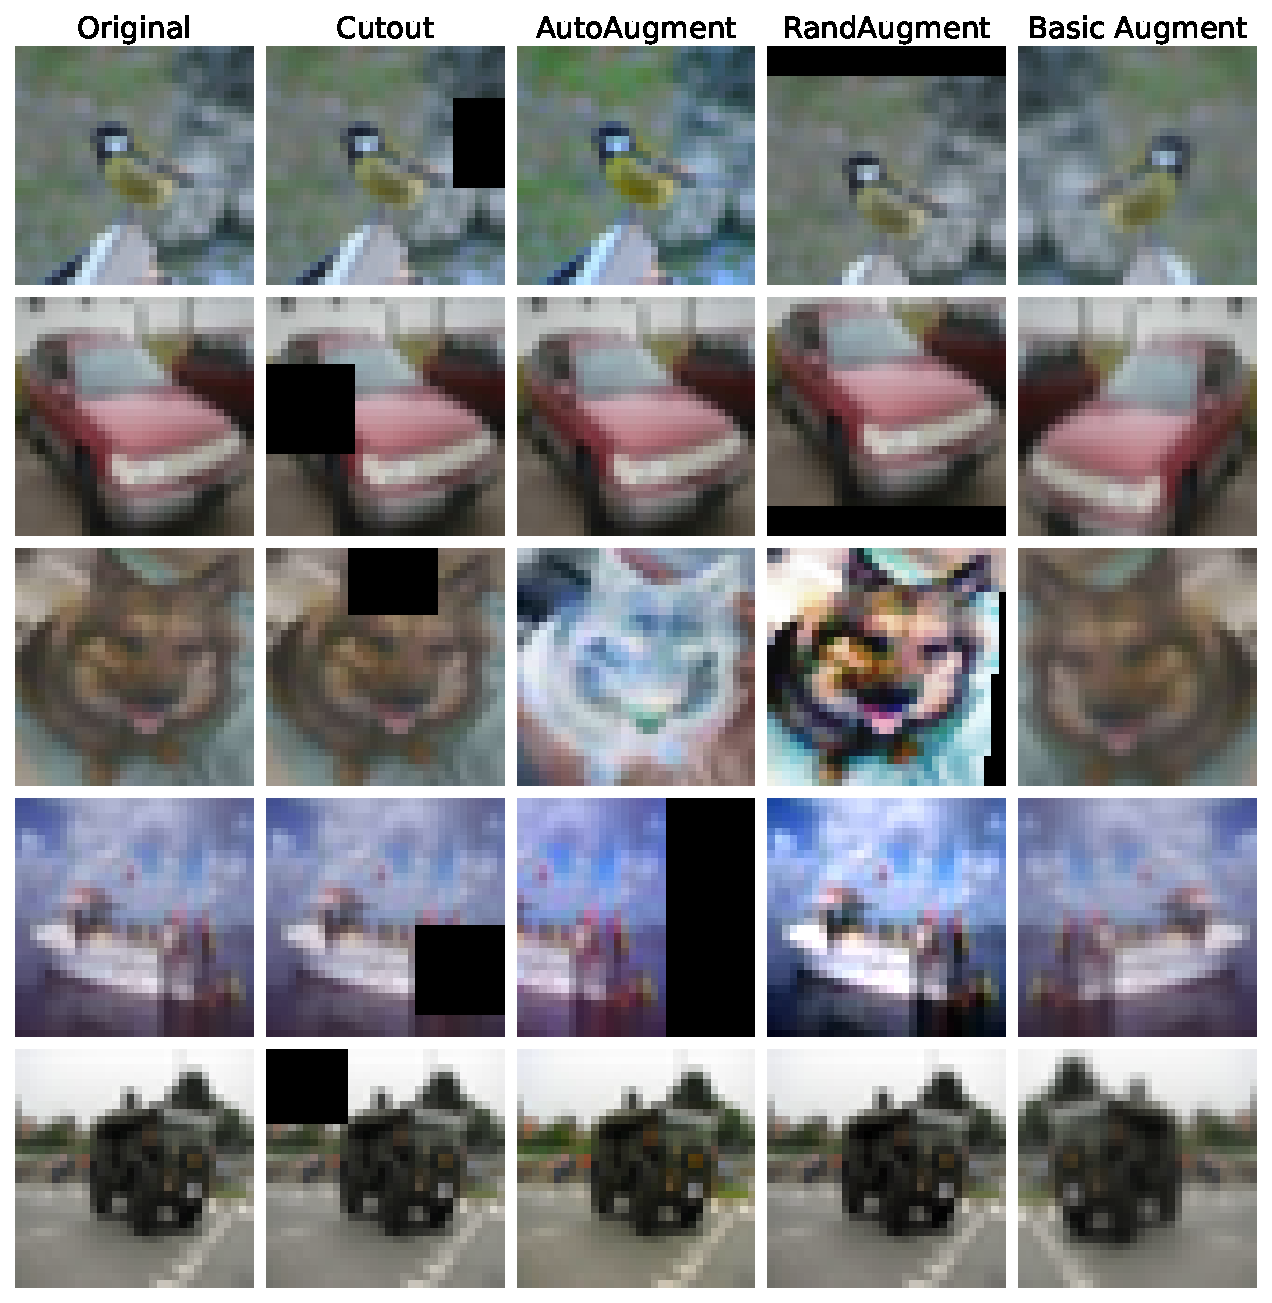
\includegraphics[width=\columnwidth]{augmentation_examples.pdf}
    \caption{Examples of data augmentation on a CIFAR-10. From left to right: Original, Cutout, AutoAugment, RandAugment, basic Augment (Crop, Flip).}
    \label{fig:example-data-aug}
\end{figure}

This lightweight augmentation pipeline provides a scalable and effective solution for addressing class imbalance, making it particularly valuable in real-world applications where data distributions are naturally skewed, such as medical diagnosis, fraud detection, and rare event prediction. By integrating efficient augmentation strategies, this approach improves fairness, accuracy, and generalization in classification models while maintaining a practical balance between performance and computational cost.

% \begin{algorithm}[htb]
% \SetAlgoLined
% \textbf{Required:} Dataset $D = \{(\mathbf{x}_i, y_i)\}_{i=1}^n$, model with parameter $\theta$\;
% \textbf{Hyperparameters:} $\alpha$, $\gamma$, batch size $M$, learning rate $\delta$, $\beta$ for \textit{effective number}\;
% Compute number of samples $n_c$ for each class $c$\;
% Compute class weight $w_c = \frac{1 - \beta}{1 - \beta^{n_c}}$ for each class\;
% Normalize weight: $w_c \gets \frac{w_c}{\sum_k w_k}$\;
% Initialize model parameter $\theta$\;
% \While{training}{
%   Sample batch $\{(\mathbf{x}_i, y_i), (\mathbf{x}_j, y_j)\}_{m=1}^M$ from $D$ using WeightedRandomBatchSampler or WeightedFixedBatchSampler with $\alpha$\;
%   Sample $\lambda_x \sim \mathit{Beta}(\gamma, \gamma)$\;
%   \For{$m = 1$ to $M$}{
%     (a) Obtain mixed input: $\tilde{\mathbf{x}}_m = \lambda_\mathbf{x} \mathbf{x}_i + (1 - \lambda_\mathbf{x}) \mathbf{x}_j$\;
%     (b) Compute label mixing coefficient $\lambda_y = \lambda_x$ or re-compute based on logits margin\;
%     (c) Mix label: $\tilde{y}_m = \lambda_y y_i + (1 - \lambda_y) y_j$\;
%   }
%   Compute loss: $\mathcal{L}(\theta) = \frac{1}{M} \sum_{m=1}^{M} w_{\tilde{y}_m} \cdot L(f(\tilde{\mathbf{x}}_m), \tilde{y}_m)$\;
%   Update parameters: $\theta \gets \theta - \delta \nabla_\theta \mathcal{L}(\theta)$\;
% }
% % \caption{Light-weight data augmentation framework training algorithm.}
% \end{algorithm}

\begin{algorithm}[htb]
\SetAlgoLined

\textbf{Required:} Dataset $D = \{(\mathbf{x}_i, y_i)\}_{i=1}^n$, model with parameter $\theta$\;
\textbf{Hyperparameters:} $\alpha$, $\gamma$, batch size $M$, learning rate $\delta$, $\beta$ for \textit{effective number}\;

Compute number of samples $n_c$ for each class $c$\;
Compute class weight $w_c = \frac{1 - \beta}{1 - \beta^{n_c}}$ for each class\;
Normalize weight: $w_c \gets \frac{w_c}{\sum_k w_k}$\;
Initialize model parameter $\theta$\;

\While{training}{
  Sample batch $\{(\mathbf{x}_i, y_i),(\mathbf{x}_j, y_j)\}_{m=1}^M$ from $D$ using 
  \texttt{WeightedRandomBatchSampler} or \texttt{WeightedFixedBatchSampler} with $\alpha$\;

  Sample $\lambda_x \sim \mathrm{Beta}(\gamma,\gamma)$\;

  \For{$m = 1$ to $M$}{
    Obtain mixed input:
    $\tilde{\mathbf{x}}_m = \lambda_x \mathbf{x}_i + (1-\lambda_x)\mathbf{x}_j$\;

    Compute label mixing coefficient $\lambda_y = \lambda_x$, or re-compute based on logits margin\;

    Mix label:
    $\tilde{y}_m = \lambda_y y_i + (1-\lambda_y)y_j$\;
  }

  Compute loss:
  $\mathcal{L}(\theta) =
  \frac{1}{M}\sum_{m=1}^{M}
  w_{\tilde{y}_m}
  L\bigl(f(\tilde{\mathbf{x}}_m),\tilde{y}_m\bigr)$\;

  Update parameters:
  $\theta \gets \theta - \delta \nabla_\theta \mathcal{L}(\theta)$\;
}

\caption{Light-weight data augmentation framework training algorithm.}
\label{alg:lightweight-augmentation}
\end{algorithm}

The effectiveness of the proposed approaches lies in their ability to balance computational efficiency and discriminative feature representation. Unlike naive resampling methods that may distort the intrinsic data distribution, these training strategies—particularly re-weighting and mixup-based augmentation—offer robust alternatives by leveraging class-balanced weighting and convex sample interpolation. While such methods enhance generalization under class imbalance, they also require careful tuning of hyperparameters (\textit{e.g., mixup intensity, weighting schedule}) to avoid label noise and maintain semantic consistency across classes.

\vspace{0.5em}
\noindent
The standard cross-entropy loss for a model output $\mathbf{z}_i \in \mathbb{R}^C$ (\textit{the logits}) and a target class $c \in \{1, \dots, C\}$ is defined as:
{\footnotesize
\begin{equation}
\mathcal{L}_{\mathrm{CE}}
= -\frac{1}{N} \sum_{i=1}^{N}
    \log \frac{\exp(z_{i, c})}{\sum_{j=1}^{C} \exp(z_{i, j})}
= -\frac{1}{N} \sum_{i=1}^{N}
    \log \big( \phi(\mathbf{z}_i)_{c} \big),
\end{equation}}
where $\phi(\cdot)$ denotes the softmax mapping from logits to class probabilities.

% ---------------------------------------------------------------------
\subsection{Empirical Risk Minimization (ERM)}
ERM treats all training samples equally without considering label imbalance. This serves as the baseline for comparison against adaptive re-weighting or augmentation strategies.

% ---------------------------------------------------------------------
\subsection{Deferred Re-Weighting (DRW):}
DRW mitigates imbalance by assigning class-dependent weight that evolve over training epochs.  
For each class $c$, a weight inversely proportional to its effective number of samples is defined as equation (3) and (4).
Weight is normalized to maintain comparability across classes:
\begin{equation}
w_c \leftarrow \frac{C w_c}{\sum_{j=1}^{C} w_j}.
\end{equation}
The weighted cross-entropy loss becomes:
\begin{equation}
\mathcal{L}_{\mathrm{DRW}}
= -\frac{1}{N} \sum_{i=1}^{N}
    w_{c} \log \big( \phi(\mathbf{z}_i)_{c} \big).
\end{equation}
By gradually activating class weight during training, DRW enables stable feature learning in early epochs and better balance in later stages.

% ---------------------------------------------------------------------
\subsection{Mixup:}
Mixup enhances generalization by linearly interpolating samples and labels such as Eq. \eqref{mixup_x} and 
Eq. \eqref{mixup_y} from section \ref{Mixup_interpolation}.
The loss is a convex combination of cross-entropies:
\begin{equation}
\mathcal{L}_{\mathrm{Mixup}}
= \lambda \, \mathcal{L}_{\mathrm{CE}}(\mathbf{z}, y_i)
+ (1 - \lambda) \, \mathcal{L}_{\mathrm{CE}}(\mathbf{z}, y_j),
\end{equation}
where $\mathbf{z}$ is the model output for the mixed input $\tilde{\mathbf{x}}$.  
Mixup smooths class boundaries and reduces overfitting by enforcing locally linear decision regions.

% ---------------------------------------------------------------------
\subsection{Imbalanced Lightweight Hybrid (ILWH) Loss:}
The ILWH objective integrates the Mixup formulation from Eq. \eqref{mixup_x} and 
Eq. \eqref{mixup_y} with the DRW scheme to achieve both data interpolation and adaptive class balancing.

\paragraph{Deferred class weight.}
Let $n_c$ denote the number of samples in class $c$. The normalized class weight is defined as:
\begin{equation}
w_c(\beta) = \frac{1 - \beta}{1 - \beta^{n_c}}, \qquad
\hat{w}_c(\beta) = \frac{C \, w_c(\beta)}{\sum_{k=1}^{C} w_k(\beta)}.
\end{equation}

\paragraph{ILWH loss}
Given the mixed samples $(\tilde{\mathbf{x}}, \tilde{\mathbf{y}})$ obtained as previously described and the corresponding model outputs $\mathbf{z}_i$, the overall batch objective is:
\begin{align}
&\mathcal{L}_{\mathrm{ILWH}}
= \frac{1}{N} \sum_{i=1}^{N}
\Big[
    \lambda \, \hat{w}_{c}(\beta) \,
        \big(-\log \phi(\mathbf{z}_i)_{y_i}\big) \nonumber \\ 
        &\quad \quad \quad \quad + (1 - \lambda) \,
        \hat{w}_{c}(\beta) \,
        \big(-\log \phi(\mathbf{z}_i)_{y_j}\big)
\Big], \\
&=\lambda \, \hat{w}_{c}(\beta) \,\mathcal{L}_{\mathrm{CE}}(\mathbf{z}, y_i) + (1 - \lambda) \, \hat{w}_{c}(\beta) \,\mathcal{L}_{\mathrm{CE}}(\mathbf{z}, y_j).
\end{align}

where $\lambda \sim \mathrm{Beta}(\gamma, \gamma)$ controls the interpolation strength, 
and $\mathcal{L}_{\mathrm{CE}}(\mathbf{z}, y_i)$ denotes the cross-entropy loss 
between the model output $\mathbf{z}$ and target label $y_i$.  

\vspace{0.5em}
\noindent
In all cases, the softmax operator $\phi(\cdot)$ transforms logits into class probabilities:
\begin{equation}
\phi(\mathbf{z})_c = \frac{\exp(z_c)}{\sum_{j=1}^{C} \exp(z_j)}.
\end{equation}

Moreover, we are also conducting further investigations to determine the optimal timing and conditions to apply augmentation techniques. Understanding\textit{ when and how} to introduce data augmentation is crucial, as different augmentation strategies may yield varying levels of effectiveness depending on the dataset characteristics, model architecture, and training dynamics. Our objective is to identify the most suitable augmentation approach for each specific method, ensuring that augmentation is neither underutilized nor excessively applied in ways that might introduce noise or degrade model performance. By systematically analyzing augmentation placement within the training pipeline, we aim to develop a \textit{more adaptive and context-aware augmentation strategy}, enabling better generalization and performance across diverse machine learning applications.

\subsection{Data Augmentation Approach}
We investigate the effectiveness of lightweight data augmentation methods: \textit{Cutout}, \textit{AutoAugment} and \textit{RandAugment}, for enhancing model generalization in the context of imbalance learning. These methods are selected due to their proven performance in previous studies, ease of implementation, and computational efficiency. An example of the effect of these techniques is shown in \ref{fig:example-data-aug}.

\subsubsection{AutoAugment}
AutoAugment~\cite{cubuk2018autoaugment} automatically searches for optimal augmentation policies to improve the validation accuracy of neural networks. Each augmentation policy comprises several sub-policies, each consisting of two sequential augmentation operations drawn from a predefined set. Specifically, a sub-policy \(S\) is defined by two augmentation operations (e.g., \textit{Shear, Rotate, Invert}): A probability associated with applying each operation and a magnitude indicating the strength of each operation.

AutoAugment formulates the search for optimal policies as a discrete optimization problem. Specifically, a controller, implemented as a recurrent neural network, samples augmentation sub-policies to form augmentation strategies. A child neural network is trained using these sampled policies and evaluated on a validation set. Validation accuracy serves as a reward signal that guides the search for policies using reinforcement learning, also known as policy gradient methods. Remarkably, AutoAugment has achieved state-of-the-art performance on datasets such as SVHN-10, CIFAR-10, CINIC-10, CIFAR-100, and TinyImageNet-200.
% \ha{the following sentence seems to be disconnected to the paragraph above. Linguistically, learned policies => not understandable}
% Although the search can be computationally expensive, learned policies have shown strong transferability between datasets, reducing the overall computational demand in practice.

\subsubsection{RandAug}
RandAugment~\cite{cubuk2019randaugment} addresses the computational complexity associated with AutoAugment by drastically reducing the augmentation search space and eliminating the separate proxy task. It uniformly applies random augmentation transformations with just two interpretable hyperparameters:
\begin{itemize}
    \item $N$: the number of augmentation operations applied sequentially.
    \item $M$: the global magnitude applied uniformly across transformations.
\end{itemize}

RandAugment randomly selects $N$ transformations from a predefined set (\textit{e.g., Rotate, TranslateX, Solarize, Color}), applying them sequentially at magnitude $M$. The simplified search space significantly reduces computational complexity from more than $10^{32}$ possibilities in AutoAugment to only $10^2$ possibilities, enabling straightforward grid searches for hyperparameter optimization~\cite{cubuk2019randaugment}.

RandAugment achieves competitive or superior performance compared to AutoAugment on standard benchmarks such as SVHN-10, CIFAR-10, CINIC-10, CIFAR-100, and TinyImageNet-200 while drastically reducing the computational resources required.

\subsubsection{Cutout}
\label{subsec:cutout}
\textit{Cutout} is a lightweight regularization method where a contiguous rectangular patch is removed (\textit{i.e., zeroed out}) from each training image at a random location~\cite{devries2017cutout}. This procedure generates partially occluded samples that effectively expand the diversity of the training set. Unlike typical dropout variants, \textit{Cutout} is applied directly to the input image rather than intermediate features. As a result, downstream feature maps corresponding to the masked region are forced to focus on contextual information surrounding the missing patch, helping the model rely on broader cues in the data~\cite{devries2017cutout}.

Suppose each training image has spatial dimensions of H$\times$ W. \textit{Cutout} selects a random center pixel \((c_x, c_y)\) within the image and replaces all pixels in a square patch of side length \(M\) (\textit{the primary hyperparameter of Cutout}) with zeros. Parts of the square lying outside the image boundaries are simply discarded. For best performance, it is recommended to first normalize the image about zero to minimize distributional shifts introduced by zero-pixels. Furthermore, the value of \(M\) is typically empirically validated depending on the resolution and complexity of the dataset~\cite{devries2017cutout}.

% Cutout offers three key benefits. First, by simulating occluded objects, it encourages the network to learn from less discriminative regions and thus become more robust to real-world occlusions. Second, it can be easily combined with common data augmentation techniques such as flipping or cropping, as well as methods like AutoAugment or RandAugment~\cite{cubuk2018autoaugment, cubuk2019randaugment}. Finally, it is straightforward to implement, typically requiring only a few lines of code during data loading.


\subsection{Data Sampling Approach}

To establish a baseline for analyzing the effectiveness of batch sampling approaches, we implemented a standard Empirical Risk Minimization (ERM) strategy without any batch sampling interventions. This baseline provides a comparison point for assessing the impact of different sampling methods. The model was trained on an imbalanced dataset, and performance metrics such as accuracy, precision, and F1-score were recorded. The results highlighted the challenges of training on imbalanced datasets, where minority class accuracy and generalization were significantly lower than those of majority classes.

We conducted two primary batch sampling methods to address the imbalance in class distributions:

\begin{itemize}
    \item \textit{Weighted Random Batch Sampler (WRBS)} This method samples with replacement based on dynamically computed weight for each class. It probabilistically selects samples according to their assigned weight, ensuring diversity in class representation within each batch, but allowing variability in batch composition across training epochs.

    \item \textit{Weighted Fixed Batch Sampler (WFBS)} This method enforces strict proportions of samples per class in each batch. By ensuring a fixed number of samples from each class, WFBS maintains consistent class representation across batches, which is critical for scenarios requiring precise balancing.
\end{itemize}
% put this macro in your preamble

\paragraph{Alpha Parameter $\alpha$} Both samplers incorporate an adjustable parameter $\alpha$ to balance between:
\begin{itemize}
    \item \textit{Training population class distribution:} The weight is proportional to the original class sizes in the dataset.
    \item \textit{Uniform distribution:} All classes are equally represented.
\end{itemize}

The combined weight \( w_i \) for each class is computed as:
\begin{equation}
w_i = \alpha \cdot w_i^{u} + (1 - \alpha) \cdot w_i^{o},
\end{equation}
where: $w_i^{u} = \frac{1}{C}$: \text{uniform weight}, $w_i^{o} = \frac{n_i}{N}$: \text{original weight}, and $\alpha \in [0, 1]$.
Here, \(C\) is the total number of classes, \(n_i\) is the number of samples in class \(i\), and \(N\) is the total number of samples in the dataset. \(\alpha = 0\) relies entirely on the original class distribution, while \(\alpha = 1\) creates a uniform distribution. Intermediate values of \(\alpha\) strike a balance between the two.

% \ha{What is difference between eq 3 and eq 6? - \textbf{Duy}: duplicated content - will remove one of 2}

\paragraph{Hypothesis from Baseline}
The baseline results demonstrated severe bias towards the majority classes, leading to suboptimal performance on minority classes. Based on this, our hypothesis is as follows:
\begin{itemize}
    \item Implementing \textit{Weighted Random Batch Sampler (WRBS)} will improve minority class accuracy due to its adaptive sampling strategy, but the variability in batch composition may cause fluctuations during training.
    \item Using \textit{Weighted Fixed Batch Sampler (WFBS)} will offer consistent improvement in class representation across batches, leading to more stable training and better generalization compared to WRBS.
    \item Increasing \(\alpha\) (\textit{i.e., moving towards a uniform distribution}) will enhance generalization by ensuring fair representation of minority classes but may reduce model focus on majority classes, impacting overall accuracy.
\end{itemize}

\newcommand{\valpm}[2]{%
  \ensuremath{#1\,{\scriptstyle\pm}\,#2}%
}

\begin{table*}[t]
\centering
\caption{Average top-1 validation accuracy (\%, mean $\pm$ std) of different sampling methods with different sampling parameters and  with imbalance ratio 0.01. Best results are highlighted in \textbf{bold}. \label{tab:merged_comparison}}
\setlength{\tabcolsep}{5pt}
\begin{tabular}{l c cc cc cc}
\toprule
\toprule
\multirow{2}{*}{\textbf{Sampling Method}} & \multirow{2}{*}{$\alpha$} 
& \multicolumn{2}{c}{\textbf{CIFAR-10}} 
& \multicolumn{2}{c}{\textbf{SVHN-10}} 
& \multicolumn{2}{c}{\textbf{CIFAR-100}} \\
\cmidrule(lr){3-4} \cmidrule(lr){5-6} \cmidrule(lr){7-8}
& & ERM & ILWH (Ours) & ERM & ILWH (Ours) & ERM & ILWH (Ours) \\
\midrule
\midrule
\multirow{3}{*}{\textbf{WRBS}}
 & $\alpha=0.5$ & \valpm{71.76}{0.24} & \valpm{81.66}{0.42} & \textbf{\valpm{82.79}{0.29}} & \valpm{81.69}{0.16} & \valpm{38.59}{0.22} & \textbf{\valpm{47.82}{0.38}} \\
 & $\alpha=0.7$ & \valpm{71.97}{0.61} & \valpm{81.74}{0.17} & \valpm{81.44}{0.18} & \valpm{81.46}{0.42} & \valpm{37.56}{0.24} & \valpm{46.15}{0.41} \\
 & $\alpha=1.0$ & \valpm{71.65}{0.62} & \textbf{\valpm{82.41}{0.21}} & \valpm{82.79}{0.25} & \valpm{81.20}{0.36} & \valpm{35.34}{0.58} & \valpm{44.88}{0.52} \\
\midrule
\multirow{3}{*}{\textbf{WFBS}}
 & $\alpha=0.5$ & \valpm{71.93}{0.61} & \valpm{82.09}{0.38} & \valpm{80.56}{0.17} & \valpm{82.00}{0.31} & \valpm{37.12}{0.26} & \textbf{\valpm{45.79}{0.35}} \\
 & $\alpha=0.7$ & \valpm{71.61}{0.64} & \textbf{\valpm{82.20}{0.18}} & \valpm{81.16}{0.57} & \valpm{81.52}{0.32} & \valpm{36.48}{0.30} & \valpm{44.93}{0.42} \\
 & $\alpha=1.0$ & \valpm{71.95}{0.65} & \valpm{81.95}{0.23} & \valpm{80.95}{0.18} & \textbf{\valpm{82.56}{0.25}} & \valpm{34.85}{0.61} & \valpm{43.71}{0.47} \\
\midrule
\textbf{Random \cite{cheng2023smote}} 
 & -- & \valpm{71.23}{0.51} & \valpm{82.11}{0.57} & \valpm{79.97}{0.67} & \valpm{85.19}{0.32} & \valpm{38.46}{0.36} & \valpm{46.91}{0.46} \\
\bottomrule
\bottomrule
\end{tabular}
\end{table*}